% Do not edit. These are fallback values, the actual values may have been
% set by the build system elsewhere.
\providecommand\topdir{.}%
\providecommand\handoutoption{}% option, normal beamer presentation mode by default


% Optional parameters for the documentclass should be the only
% things to be changed in this file.
\documentclass[
%%%%%%%%%% Start of customizable section %%%%%%%%%%
english,
ngerman,
10pt,%             supported values: 10pt, 11pt, 12pt
aspectratio=169,%  common values: 169, 1610, 43
%%%%%%%%%% End of customizable section %%%%%%%%%%
\handoutoption
]{beamer}


\usepackage{etoolbox}
\newtoggle{prebuiltslides}
\ifdefined\prebuiltslides
  \toggletrue{prebuiltslides}
\else
  \togglefalse{prebuiltslides}
\fi

% do not change the default packages
% allow many more packages, keep this as first package
\usepackage{etex}
\usepackage{luacode}
\usepackage{luatex85}

\usepackage[ngerman,main=english]{babel}

% Do not change this file

%define colors
\usepackage{xcolor}

\usepackage{graphics}

% change document reference style
\usepackage{hyperref}

\lstset{ language=C++,
         basicstyle=\footnotesize\ttfamily, % Standardschrift
         numbers=none,               % Ort der Zeilennummern
         numberstyle=\footnotesize,          % Stil der Zeilennummern
         %stepnumber=2,               % Abstand zwischen den Zeilennummern
         numbersep=5pt,              % Abstand der Nummern zum Text
         tabsize=2,                  % Groesse von Tabs
         extendedchars=true,         %
         breaklines=true,            % Zeilen werden Umgebrochen
         keywordstyle=\color{fzjblue},
         frame=,
         keywordstyle=[1]\textbf,    % Stil der Keywords
         keywordstyle=[2]\textbf,    %
         keywordstyle=[3]\textbf,    %
         keywordstyle=[4]\textbf,   %\sqrt{\sqrt{}} %
         rulesepcolor=\color{fzjblue},
         fillcolor=\color{fzjblue},
         stringstyle=\color{red!50!brown}\ttfamily, % Farbe der String
         showspaces=false,           % Leerzeichen anzeigen ?
         showtabs=false,             % Tabs anzeigen ?
         xleftmargin=15pt,
         framexleftmargin=1pt,
         framexrightmargin=1pt,
         framexbottommargin=1pt,
         %backgroundcolor=\color{fzjblue},
         showstringspaces=false,      % Leerzeichen in Strings anzeigen ?
         nolol=true,
 }

\lstdefinelanguage
   {x64-Assembler}     % add a "x64" dialect of Assembler
   [x86masm]{Assembler} % based on the "x86masm" dialect
   % with these extra keywords:
   {morekeywords={vsubpd,vmulpd,vaddpd,vsqrtpd,vdivpd,
                  vsubps,vmulps,vaddps,vsqrtps,vdivps,
                  vmovss,vsubss,vmulss,vaddss,vsqrtss,vdivss,
                  vmovsd,vsubsd,vmulsd,vaddsd,vsqrtsd,vdivsd,
                  vmovaps,vmovapd,
                  vfmadd231ps,vfmadd231pd,
                  xmm,ymm,
                  CDQE,CQO,CMPSQ,CMPXCHG16B,JRCXZ,LODSQ,MOVSXD, %
                  POPFQ,PUSHFQ,SCASQ,STOSQ,IRETQ,RDTSCP,SWAPGS, %
                  rax,rdx,rcx,rbx,rsi,rdi,rsp,rbp, %
                  r8,r8d,r8w,r8b,r9,r9d,r9w,r9b}}
 \lstloadlanguages{% Check Dokumentation for further languages ...
         x64-Assembler,
         C,
         C++,
 }
\lstset{language=C++,
    keywordstyle=\color{fzjblue}\bfseries,
    commentstyle=\color{green!60!black},
    stringstyle=\ttfamily\color{red!50!brown},
    morekeywords={Real,Scalar}
    }
\lstset{literate=%
   *{0}{{{\color{red!20!violet}0}}}1
    {1}{{{\color{red!20!violet}1}}}1
    {2}{{{\color{red!20!violet}2}}}1
    {3}{{{\color{red!20!violet}3}}}1
    {4}{{{\color{red!20!violet}4}}}1
    {5}{{{\color{red!20!violet}5}}}1
    {6}{{{\color{red!20!violet}6}}}1
    {7}{{{\color{red!20!violet}7}}}1
    {8}{{{\color{red!20!violet}8}}}1
    {9}{{{\color{red!20!violet}9}}}1
}

%\DeclareCaptionFont{fzjblue}{\color{fzjblue}}
%\DeclareCaptionFont{fzjgray}{\color{fzjgray}}
%%  \captionsetup[lstlisting]{singlelinecheck=false, labelfont={fzjblue}, textfont={fzjblue}}


%\DeclareCaptionFont{white}{\color{white}}
%\DeclareCaptionFormat{listing}{\colorbox[cmyk]{0.09, 0.05, 0.05,0.01}{\parbox[b][1.5ex][c]{\textwidth}{\hspace{15pt}#1#2#3}}}
%%\captionsetup[lstlisting]{format=listing,labelfont=fzjblue,textfont=fzjgray, singlelinecheck=false, margin=0pt, font={sc, bf,footnotesize}}
%\captionsetup{labelformat=empty,labelsep=none}

%pgf tikz and related
\usepackage{pgf}
\usepackage{tikz}
\usepackage{fp}
\usepackage{pgfplots}

%allow environment with tikz
\usepackage{environ}

\usepackage{tikz-3dplot}

% settings for the design of tables
\arrayrulecolor{fzjblue}

% allow watermark from git hash key
\iftoggle{prebuiltslides}{
  % no git info for prebuilt slides
}{
  \usepackage{gitinfo2}
}



% add required packages inside the packages.local.tex
% additional packages you need to include should go here


% do not change the default config
% Do not change this file, all changes must go into the config.local.tex file

% prefixes the includegraphics path with these directories
\graphicspath{{Images/}{Plots/}{Figures/}}

% external config files for different packages and/or features
\newcommand{\modesuffix}{.beamer}

%beamer handout definitions
\mode<handout>{
  \usetheme{Juelich}
  \iftoggle{prebuiltslides}{
    \pgfpageslogicalpageoptions{1}{border code=}
    \pgfpagesuselayout{resize to}[
      physical paper height=\paperheight,
      physical paper width=\paperwidth]
  }{
  \pgfpagesuselayout{2 on 1}[a4paper,border shrink=5mm]
  }
  \renewcommand{\modesuffix}{.handout}
}

% use the Juelich theme for all slides in presentation mode
\mode<presentation>{
  \usetheme{Juelich}
}

%\fzjset{title=allcaps}         % to set the title in allcaps
 \fzjset{title=regular}         % to set the title regular
%\fzjset{subtitle=allcaps}      % to set the title in allcaps for short text
%\fzjset{subtitle=regular}      % to set the title regular and in a smaller font for long text
%\fzjset{part=allcaps}          % to set the part in allcaps for short text
%\fzjset{part=regular}          % to set the part regular and in a smaller font for long text
%\fzjset{frametitle=allcaps}    % to set the frametitle in allcaps for short text
 \fzjset{frametitle=regular}    % to set the frametitle regular font for long text

% define \emph as color version, no bold, slanted, italic, please
\renewcommand{\emph}[1]{\structure{#1}}

% simply incremental slides inside tikz
\tikzset{
  onslide/.code args={<#1>#2}{%
    \only<#1>{\pgfkeysalso{#2}} % \pgfkeysalso doesn't change the path
  }
}

\DeclareRobustCommand{\includetitle}[1]{
  \pdfximage{#1\modesuffix.pdf}
  \pgfmathparse{\the\pdflastximagepages}
  \foreach \x in {1,...,\pgfmathresult} {
  \setbeamertemplate{frame number}[invisible]%
  \setbeamertemplate{date}[invisible]%
  \setbeamertemplate{background canvas}{
    \includegraphics[page=\x,width=\paperwidth,height=\paperheight,keepaspectratio]{#1\modesuffix}}
  \begin{frame}\end{frame} \setbeamertemplate{background canvas}{}
  \addtocounter{framenumber}{-1} % counter will increase on every frame
  }
}

\DeclareRobustCommand{\includeframeset}[1]{
  \pdfximage{#1\modesuffix.pdf}
  \pgfmathparse{\the\pdflastximagepages}
  \foreach \x in {1,...,\pgfmathresult} {
  \setbeamertemplate{background canvas}{
    \includegraphics[page=\x,width=\paperwidth,height=\paperheight,keepaspectratio]{#1\modesuffix}}
  \begin{frame}\end{frame} \setbeamertemplate{background canvas}{}
%  \addtocounter{framenumber}{-1} % counter will increase on every frame
  }
}

\DeclareRobustCommand{\includeframeoverlay}[1]{
  \pdfximage{#1\modesuffix.pdf}
  \pgfmathparse{\the\pdflastximagepages}
  \foreach \x in {1,...,\pgfmathresult} {
  \setbeamertemplate{background canvas}{
    \includegraphics[page=\x,width=\paperwidth,height=\paperheight,keepaspectratio]{#1\modesuffix}}
  \begin{frame}\end{frame} \setbeamertemplate{background canvas}{}
  \addtocounter{framenumber}{-1} % keeps counter constant
  }
  \addtocounter{framenumber}{+1} % sets framecounter for next slide outside this group
}

% TODO copy in beamertheme-juelich template
\definecolor{fzjblack}{RGB}{0,0,0}

\usefonttheme{professionalfonts} % needed to use math symbols from fontenc

\usepackage{amsmath}
\usepackage{latexsym} % replaces amssymb

\usepackage{unicode-math} % enables \setmathfont commands
\usepackage{fontawesome} % loads fancy web symbols

\setmainfont[
  Scale=0.9,
  Extension=.ttf,
  UprightFont=*-Regular,
  BoldFont=*-Bold,
  ItalicFont=*-Italic,
  BoldItalicFont=*-BoldItalic,
  SlantedFont=*-Italic,
]{LiberationSans}

\setsansfont[
  Scale=0.9,
  Extension=.ttf,
  UprightFont=*-Regular,
  BoldFont=*-Bold,
  ItalicFont=*-Italic,
  BoldItalicFont=*-BoldItalic,
  SlantedFont=*-Italic,
]{LiberationSans}

\setmonofont[
  Scale=0.9,
  Extension=.ttf,
  UprightFont=*-Regular,
  BoldFont=*-Bold,
  ItalicFont=*-Italic,
  BoldItalicFont=*-BoldItalic,
  SlantedFont=*-Italic,
]{LiberationMono}

\unimathsetup{math-style=ISO} % french, ISO, TeX, upright

\setmathfont[Scale=1]{TeX Gyre Bonum Math}
\setmathfont[Scale=0.9,range=\mathup/{latin,Latin,num}]{LiberationSans}
\setmathfont[Scale=0.9,range=\mathit/{latin,Latin,num}]{LiberationSans-Italic}
\setmathfont[Scale=0.9,range=\mathbfup/{latin,Latin,num}]{LiberationSans-Bold}
\setmathfont[Scale=0.9,range=\mathbfit/{latin,Latin,num}]{LiberationSans-BoldItalic}
\setmathfont[Scale=1,range=\mathcal/{latin,Latin}]{jsMath-cmsy10} % loads  nice calligraph symbols
\setmathfont[Scale=1,range=\mathbb/{greek,Greek,latin,Latin,num}]{TeX Gyre Bonum Math} % loads  nice calligraph symbols

% change document reference style
\usepackage{hyperref}

%pgf tikz and related
\usepackage{pgf}
\usepackage{tikz}
\usepackage{fp}
\usepackage{pgfplots}

%allow environment with tikz
\usepackage{environ}

\usepackage{tikz-3dplot}

\pgfplotsset{compat=1.14}

\pgfplotscreateplotcyclelist{fzjblue}{
{fzjblue},
{fzjblue!80!white},
{fzjblue!70!white},
{fzjblue!60!white},
{fzjblue!50!white},
{fzjblue!40!white},
{fzjblue!30!white},
{fzjblue!20!white},
{fzjblue!10!white},
}

\pgfplotscreateplotcyclelist{fzjdiagram}{
{fzjblue},
{fzjorange},
{fzjgray!50!black},
{fzjviolet},
{fzjred},
{fzjgreen},
{fzjyellow},
{fzjlightblue},
}

\newcommand\globe{%
\hspace{0.1em}%
\tikz
\path [y=0.009ex,x=0.009ex,yscale=-1,inner sep=0pt,outer sep=0pt,fill]
    (90,90) circle (90)%
    (99,167) .. controls (128,164) and (155,142) ..
    (164,114) .. controls (166,107) and (170,96) ..
    (166,90) .. controls (160,91) and (159,109) ..
    (156,97) .. controls (155,87) and (142,82) ..
    (133,81) .. controls (131,89) and (146,83) ..
    (141,91) .. controls (136,97) and (125,103) ..
    (123,91) .. controls (123,87) and (115,80) ..
    (120,88) .. controls (121,94) and (124,107) ..
    (132,101) .. controls (137,110) and (120,115) ..
    (123,125) .. controls (119,133) and (112,141) ..
    (104,145) .. controls (92,148) and (91,132) ..
    (91,124) .. controls (91,115) and (87,106) ..
    (78,110) .. controls (72,112) and (67,111) ..
    (64,106) .. controls (60,103) and (58,99) ..
    (59,93) .. controls (58,83) and (67,77) ..
    (71,70) .. controls (63,68) and (69,57) ..
    (75,60) .. controls (70,51) and (83,49) ..
    (88,44) .. controls (95,46) and (108,42) ..
    (101,34) .. controls (97,26) and (100,47) ..
    (92,41) .. controls (88,39) and (80,37) ..
    (87,32) .. controls (93,26) and (103,29) ..
    (111,29) .. controls (118,28) and (132,30) ..
    (134,27) .. controls (127,19) and (116,16) ..
    (105,13) .. controls (91,10) and (76,11) ..
    (62,17) .. controls (55,20) and (43,22) ..
    (44,31) .. controls (47,38) and (37,50) ..
    (33,49) .. controls (32,43) and (28,38) ..
    (25,46) .. controls (18,54) and (31,66) ..
    (20,72) .. controls (10,78) and (10,91) ..
    (12,101) .. controls (14,112) and (26,115) ..
    (30,125) .. controls (37,130) and (47,134) ..
    (39,143) .. controls (32,149) and (47,154) ..
    (51,158) .. controls (65,165) and (83,170) ..
    (99,167) --
    cycle
    (124,138) .. controls (119,132) and (136,122) ..
    (129,133) .. controls (128,134) and (128,139) ..
    (124,138) --
    cycle
    (73,42) .. controls (63,39) and (81,27) ..
    (80,39) .. controls (80,41) and (75,44) ..
    (73,42) --
    cycle
    (100,77) .. controls (105,74) and (121,81) ..
    (115,72) .. controls (111,71) and (106,63) ..
    (103,69) .. controls (99,66) and (98,56) ..
    (93,60) .. controls (97,61) and (98,70) ..
    (93,64) .. controls (90,52) and (70,71) ..
    (81,70) .. controls (91,64) and (93,82) ..
    (100,77) --
    cycle
    (136,67) .. controls (138,62) and (133,52) ..
    (129,61) .. controls (131,63) and (133,77) ..
    (136,67) --
    cycle
    (123,63) .. controls (122,55) and (104,57) ..
    (112,64) .. controls (116,65) and (120,66) ..
    (123,63) --
    cycle;%
\hspace{0.25em}%
}

\lstset{ language=C++,
         basicstyle=\footnotesize\ttfamily, % Standardschrift
         numbers=none,               % Ort der Zeilennummern
         numberstyle=\footnotesize,          % Stil der Zeilennummern
         %stepnumber=2,               % Abstand zwischen den Zeilennummern
         numbersep=5pt,              % Abstand der Nummern zum Text
         tabsize=2,                  % Groesse von Tabs
         extendedchars=true,         %
         breaklines=true,            % Zeilen werden Umgebrochen
         keywordstyle=\color{fzjblue},
         frame=,
         keywordstyle=[1]\textbf,    % Stil der Keywords
         keywordstyle=[2]\textbf,    %
         keywordstyle=[3]\textbf,    %
         keywordstyle=[4]\textbf,   %\sqrt{\sqrt{}} %
         rulesepcolor=\color{fzjblue},
         fillcolor=\color{fzjblue},
         stringstyle=\color{red!50!brown}\ttfamily, % Farbe der String
         showspaces=false,           % Leerzeichen anzeigen ?
         showtabs=false,             % Tabs anzeigen ?
         xleftmargin=15pt,
         framexleftmargin=1pt,
         framexrightmargin=1pt,
         framexbottommargin=1pt,
         %backgroundcolor=\color{fzjblue},
         showstringspaces=false,      % Leerzeichen in Strings anzeigen ?
         nolol=true,
 }

\lstdefinelanguage
   {x64-Assembler}     % add a "x64" dialect of Assembler
   [x86masm]{Assembler} % based on the "x86masm" dialect
   % with these extra keywords:
   {morekeywords={vsubpd,vmulpd,vaddpd,vsqrtpd,vdivpd,
                  vsubps,vmulps,vaddps,vsqrtps,vdivps,
                  vmovss,vsubss,vmulss,vaddss,vsqrtss,vdivss,
                  vmovsd,vsubsd,vmulsd,vaddsd,vsqrtsd,vdivsd,
                  vmovaps,vmovapd,
                  vfmadd231ps,vfmadd231pd,
                  xmm,ymm,
                  CDQE,CQO,CMPSQ,CMPXCHG16B,JRCXZ,LODSQ,MOVSXD, %
                  POPFQ,PUSHFQ,SCASQ,STOSQ,IRETQ,RDTSCP,SWAPGS, %
                  rax,rdx,rcx,rbx,rsi,rdi,rsp,rbp, %
                  r8,r8d,r8w,r8b,r9,r9d,r9w,r9b}}
 \lstloadlanguages{% Check Dokumentation for further languages ...
         x64-Assembler,
         C,
         C++,
 }
\lstset{language=C++,
    keywordstyle=\color{fzjblue}\bfseries,
    commentstyle=\color{green!60!black},
    stringstyle=\ttfamily\color{red!50!brown},
    morekeywords={Real,Scalar}
    }
\lstset{literate=%
   *{0}{{{\color{red!20!violet}0}}}1
    {1}{{{\color{red!20!violet}1}}}1
    {2}{{{\color{red!20!violet}2}}}1
    {3}{{{\color{red!20!violet}3}}}1
    {4}{{{\color{red!20!violet}4}}}1
    {5}{{{\color{red!20!violet}5}}}1
    {6}{{{\color{red!20!violet}6}}}1
    {7}{{{\color{red!20!violet}7}}}1
    {8}{{{\color{red!20!violet}8}}}1
    {9}{{{\color{red!20!violet}9}}}1
}

%\DeclareCaptionFont{fzjblue}{\color{fzjblue}}
%\DeclareCaptionFont{fzjgray}{\color{fzjgray}}
%%  \captionsetup[lstlisting]{singlelinecheck=false, labelfont={fzjblue}, textfont={fzjblue}}


%\DeclareCaptionFont{white}{\color{white}}
%\DeclareCaptionFormat{listing}{\colorbox[cmyk]{0.09, 0.05, 0.05,0.01}{\parbox[b][1.5ex][c]{\textwidth}{\hspace{15pt}#1#2#3}}}
%%\captionsetup[lstlisting]{format=listing,labelfont=fzjblue,textfont=fzjgray, singlelinecheck=false, margin=0pt, font={sc, bf,footnotesize}}
%\captionsetup{labelformat=empty,labelsep=none}

% settings for the design of tables
\arrayrulecolor{fzjblue}

\part{How To Do Bibliographies}
\begin{frame}
    \frametitle{How to Do References}
    \begin{itemize}
      \item My talk is interesting \cite{ref1}.
      \item But this paper shows how it is really done \cite{ref2}.
      \item Wow, these guys did stupid things \cite{ref3}.
      \item Cite figures in the caption below, or in the text aside.
      \item Put your references in \texttt{references.bib}
    \end{itemize}
\end{frame}

\section{References}
\begin{frame}[allowframebreaks]
\frametitle{References}
    \tiny{\bibliographystyle{alpha}}
    %\tiny{\bibliographystyle{unsrt}}
    \bibliography{references}
\end{frame}



% add required configuration inside the config.local.tex
% please put additional configuration here, if needed


% ensure that separately built slides don't have any footer, yet
\iftoggle{prebuiltslides}{\setbeamertemplate{footer element1}{}
\setbeamertemplate{footer element2}{}
\setbeamertemplate{footer element3}{}
\setbeamertemplate{footer element4}{}
}{}


% \setmathfont{Latin Modern Math}
% \setmathfont{TeX Gyre Termes Math}[range=bb]
% \DeclareMathAlphabet{\mathcal}{OMS}{cmsy}{m}{n}

\begin{document}

% \verb listings \tt ttfamily

% Measure size
% \begin{tikzpicture}
% \foreach \x in {-7,...,7}
% {
%   \foreach \y in {-2...,2}
%   {
%     \node (0) at (\x,\y) {\x,\y};
%   }
% }
% \end{tikzpicture}

% Hello world!
% \begin{frame}
% \frametitle{Hello world! t.miethlinger}
% \end{frame}

\includetitle{Slides/title}

\part{Introduction}
\makepart

\begin{frame}
\frametitle{About me}
\framesubtitle{(Thomas Miethlinger)}
\begin{columns}[T]
 \begin{column}{.35\textwidth}
 \begin{itemize}
  \item Study: Master Physics
  \item Johannes Kepler University of Linz
  \item Institute for Theoretical Physics \\ Department: Many Particle Systems \\
        Research:
        \begin{itemize}
         \item Quantum fluids
         \item Complex fluids
         \item Non-equilibrium statistical mechanics
        \end{itemize}
\end{itemize}
 \end{column}
 \hfill
 \begin{column}{.65\textwidth}
 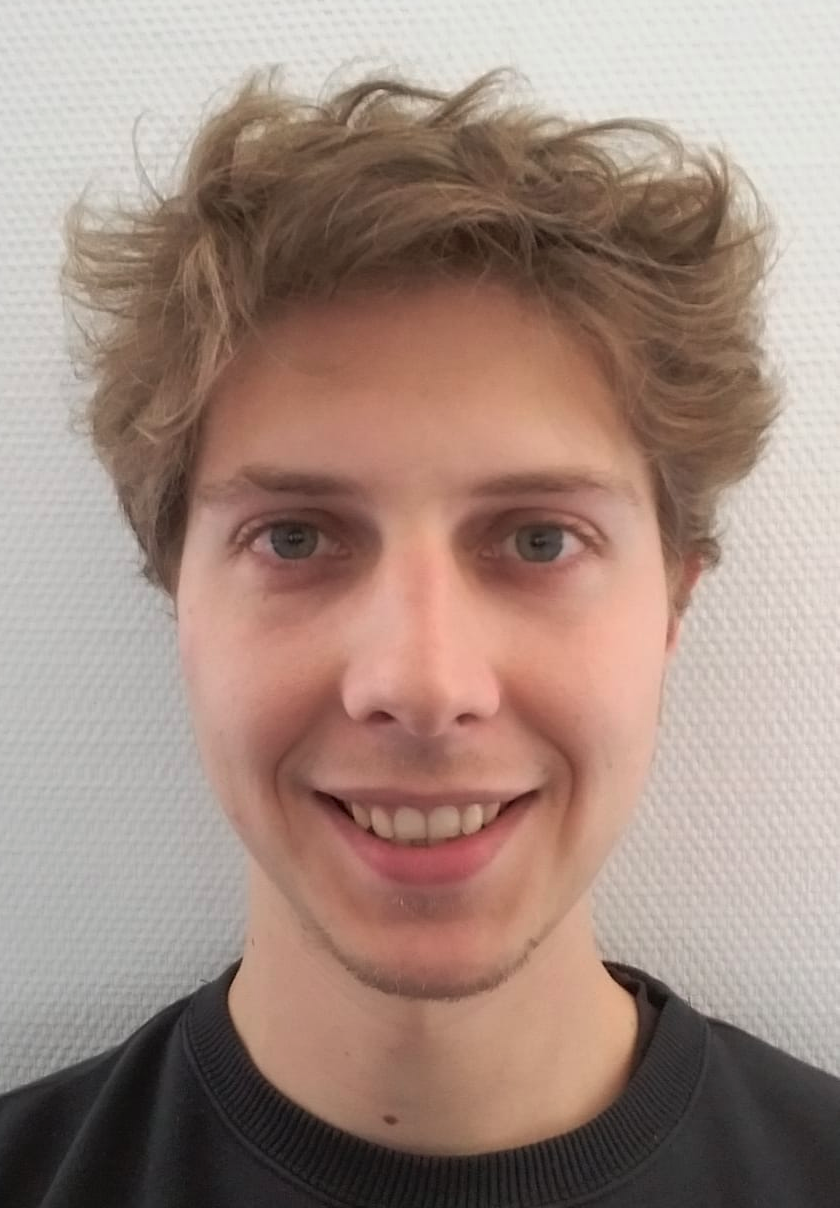
\includegraphics[width=0.287\textwidth]{photo_me.png}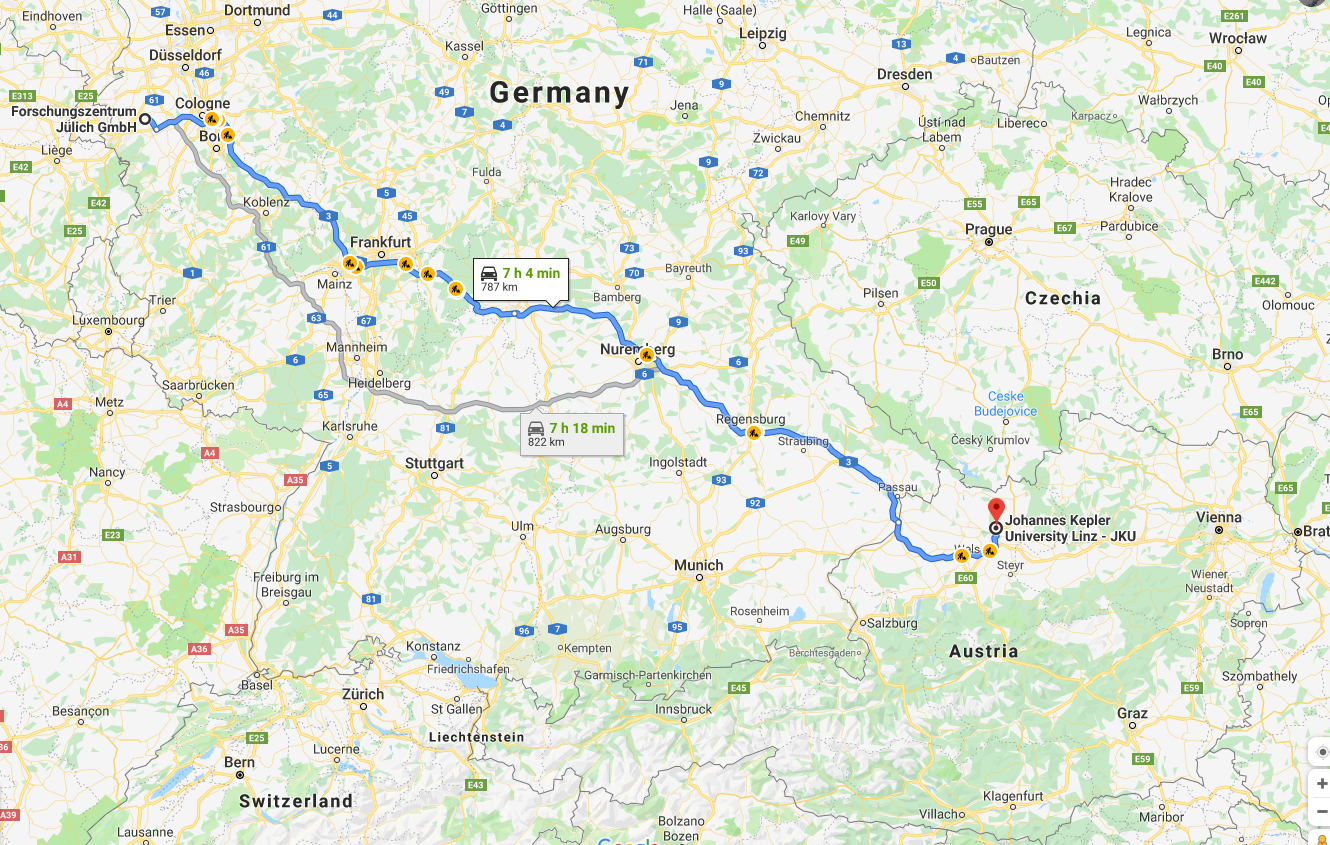
\includegraphics[width=0.65\textwidth]{fzj_jku.png}
 \end{column}
\end{columns}
\end{frame}

\begin{frame}
\frametitle{About the Supervisors}
\begin{columns}[T]
 \begin{column}{.5\textwidth}
  \begin{itemize}
  \item Supervisor: Dr. Edoardo Di Napoli
  \item Co-Supervisor: Dr. Xinzhe Wu
  \item SimLab Quantum Materials
  \item Research:
    \begin{itemize}
    \item Development and maintenance of numerical libraries
    \item Design and implementation of high-performance algorithms
    \item Development of new mathematical and computational models within a methodological framework
    \end{itemize}
    in the scope of computational materials science and quantum materials.
  \end{itemize}
 \end{column}
 \begin{column}{.5\textwidth}
 \begin{center}
  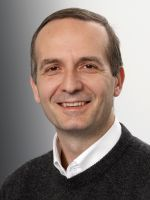
\includegraphics[width=0.4\textwidth]{di_napoli_e.jpg}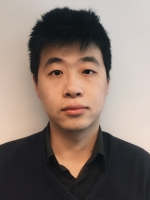
\includegraphics[width=0.4\textwidth]{wu_xin.jpg}
 \end{center}
 \end{column}
\end{columns}


\end{frame}

\part{Introduction to HPX}
\makepart

\begin{frame}
\frametitle{Current situation in high performance computing (HPC)}
Currently, speed-up in computing does not stem from higher CPU frequency, but increased parallelism.
However, we already face the following challenges in HPC:
\begin{itemize}
  \item Ease of programming
  \item Inability to handle dynamically changing workloads
  \item Scalability
  \item Efficient utilization of system resources
\end{itemize}
\(\implies\) a need for a new execution model: ParalleX, which is implemented by HPX
\end{frame}

\begin{frame}
\frametitle{ParalleX}
ParalleX is a new parallel execution model that offers an alternative to the conventional computation models(e.g. message passing):
\begin{itemize}
  \item Split-phase transaction model
  \item Message-driven
  \item Distributed shared memory
  \item Multi-threaded
  \item Futures synchronization
  \item Local Control Objects (LCOs)
  \item ...
\end{itemize}
ParalleX focuses on latency hiding instead of latency avoidance.
\end{frame}

\begin{frame}
\frametitle{About HPX}
\begin{itemize}
  \item High Performance ParalleX (HPX) is the first runtime system implementation of the ParalleX execution model.
  \item Development: STE||AR group \\ Louisiana State University \\ LSU Center for Computation and Technology
  \item Released as open source under the Boost Software License
  \item Current version: HPX V1.3.0, released on 23.05.2019
  \item Aims to be a \textbf{C++ standards conforming implementation} of the Parallelism and Concurrency proposals for C++ 17/20/23/...
  \item This means: HPX is a C++ library that supports \textbf{dynamic adaptive resource management} and \textbf{lightweight task programming and scheduling} within the context of a \textbf{global address space}. 
\end{itemize}
\end{frame}

\begin{frame}
\frametitle{On learning HPX}
\framesubtitle{An opinion of a non-CS/HPC student}
Learning curve on of HPX is quite steep - in the first days quite some dedication, effort and endurance is needed\footnote{\color{fzjblue} \href{https://github.com/STEllAR-GROUP/tutorials/blob/master/hlrs2017/session1/README.md}{Why is the HPX code repo so big and complicated?}}.
\begin{itemize}
  \item Probably the easiest way in the beginning: watch
    \color{fzjblue}\href{https://www.youtube.com/playlist?list=PL1tk5lGm7zvSXfS-sqOOmIJ0lFNjKze18}{this nice playlist}
    \color{black} in 1.25x speed on the Youtube channel of
    \color{fzjblue}\href{https://www.youtube.com/user/cscsch}{cscsch}
    \color{black}(Swiss National Supercomputing Centre)
  \item Be aware that the
    \color{fzjblue}\href{https://stellar-group.github.io/hpx/docs/sphinx/latest/html/api.html}{API reference}
    \color{black}is not complete
  \item Be aware that there exist at least 5 different ``Hello, World!'' examples\footnote{Paths are with respect to \color{fzjblue}\url{https://github.com/STEllAR-GROUP/}\color{black}}:
  \begin{itemize}
    \item hpx/examples/hello\_world\_component/*: 3 files; 28, 30 \& 55 lines
    \item hpx/examples/quickstart/hello\_world\_1.cpp; 22 lines
    \item hpx/examples/quickstart/hello\_world\_2.cpp; 24 lines
    \item hpx/examples/quickstart/hello\_world\_distributed.cpp; 156 lines
    \item tutorials/examples/01\_hello\_world/hello\_world.cpp; 71 lines
  \end{itemize}
\end{itemize}
\end{frame}

\begin{frame}
\frametitle{HPX: Tasks and Threads}
\begin{itemize}
 \item HPX: Task-based parallelism
 \item Split up big problem into smaller tasks
 \item Tasks are worked off as HPX (lightweight) Threads by the OS Threads
 \item Task size is crucial: not too small and not too big
 \item Number of tasks can even be as high as \(\mathcal{O}(10^8)\)
\end{itemize}
\vspace{0.3cm}
\begin{center}
\begin{tikzpicture}[
x=1cm,
y=1cm,
tasknode/.style={rectangle, draw=fzjblue!60, fill=fzjblue!5, very thick, minimum height=1cm},
]
\node at (-3cm,2cm) {Tasks too large};
\node[tasknode] at (-5cm  +0cm,0cm) [draw, thick, minimum width=2cm] {\(T_1\)};
\node[tasknode] at (-5cm  +2cm,0cm) [draw, thick, minimum width=2cm] {\(T_3\)};
\node[tasknode] at (-5cm  +4cm,0cm) [draw, thick, minimum width=2cm] {\(T_5\)};
\node[tasknode] at (-5cm+0.1cm,1cm) [draw, thick, minimum width=2.2cm] {\(T_2\)};
\node[tasknode] at (-5cm+2.2cm,1cm) [draw, thick, minimum width=2.2cm] {\(T_4\)};

\node at (3,2) {Right task size};
\node[tasknode] at (+1,0) [draw, thick, minimum width=1cm] {\(T_1\)};
\node[tasknode] at (+2,0) [draw, thick, minimum width=1cm] {\(T_3\)};
\node[tasknode] at (+3.2,1) [draw, thick, minimum width=1cm] {\(T_5\)};
\node[tasknode] at (+1.1,1) [draw, thick, minimum width=1.2cm] {\(T_2\)};
\node[tasknode] at (+2.2,1) [draw, thick, minimum width=1.2cm] {\(T_4\)};

\node[tasknode] at (3.05,0) [draw, thick, minimum width=1.1cm] {\(T_6\)};
\node[tasknode] at (4.1,0) [draw, thick, minimum width=1.1cm] {\(T_7\)};
\node[tasknode] at (5.1,0) [draw, thick, minimum width=1cm] {\(T_8\)};
\node[tasknode] at (4.3,1) [draw, thick, minimum width=1.2cm] {\(T_9\)};
% \node[tasknode] at (+2.1,1) [draw, thick, minimum width=1.05cm] {\(T_{10}\)};
% \node[tasknode] at (+2.1,1) [draw, thick, minimum width=1.05cm] {\(T_{11}\)};
\end{tikzpicture}
\end{center}
\end{frame}

\begin{frame}
\frametitle{Comparison of HPX and OpenMP}
\begin{center}
\begin{tabular}{ |c|c| } 
 \hline
 HPX & OpenMP \\
 \hline
 C++ library & Compiler extension to C and Fortran \\
 Core language: \texttt{hpx::C++} & \texttt{\#pragma omp} directives \\
 Task-based parallelism & Parallel regions (fork-join model) \\
 \hline
\end{tabular}
\end{center}
\vspace{0.3cm}
\begin{center}
\begin{tikzpicture}[
initnode/.style={circle, draw=fzjgreen!60, fill=fzjgreen!5, very thick, minimum size=5mm},
masternode/.style={rectangle, draw=fzjred!60, fill=fzjred!5, very thick, minimum size=5mm},
slavenode/.style={rectangle, draw=fzjblue!60, fill=fzjblue!5, very thick, minimum size=5mm},
]
\node[initnode]      at (-5, -1) {S};
\node[slavenode]     at (-4,  1) {2};
\node[slavenode]     at (-4,  0) {1};
\node[slavenode]     at (-4, -1) {0};
\node[slavenode]     at (-3,  1) {2};
\node[slavenode]     at (-3,  0) {1};
\node[slavenode]     at (-3, -1) {0};
\node[slavenode]     at (-2,  1) {2};
\node[slavenode]     at (-2,  0) {1};
\node[slavenode]     at (-2, -1) {0};
\node[initnode]      at (-1, -1) {E};
\draw[->] (-5+0.31,  -1) -- (-4-0.27, -1);
\draw[->] (-4.5,  1) -- (-4-0.27,  1);
\draw[->] (-4.5,  0) -- (-4-0.27,  0);
\draw[->] (-4.5, -1) -- (-4-0.27, -1);
\draw[-]  (-4.5, -1) -- (-4.5, 1);
\draw[->] (-4+0.27,  1) -- (-3-0.27,  1);
\draw[->] (-4+0.27,  0) -- (-3-0.27,  0);
\draw[->] (-4+0.27, -1) -- (-3-0.27, -1);
\draw[->] (-3+0.27,  1) -- (-2-0.27,  1);
\draw[->] (-3+0.27,  0) -- (-2-0.27,  0);
\draw[->] (-3+0.27, -1) -- (-2-0.27, -1);
\draw[->] (-2+0.27,  1) -- (-1.5,  1);
\draw[->] (-2+0.27,  0) -- (-1.5,  0);
\draw[-]  (-1.5, -1) -- (-1.5, 1);
\draw[->] (-2+0.27,  -1) -- (-1-0.31, -1);

\node[initnode]      at (1, -1) {S};
\node[masternode]    at (2, -1) {0};
\node[masternode]    at (3, -1) {0};
\node[slavenode]     at (3, -0) {1};
\node[slavenode]     at (3,  1) {2};
\node[masternode]    at (4, -1) {0};
\node[initnode]      at (5, -1) {E};
\draw[->] (1+0.31, -1) -- (2-0.27, -1);
\draw[->] (2+0.27, -1) -- (3-0.27, -1);
\draw[->] (2.5,  0) -- (3-0.27,  0);
\draw[->] (2.5,  1) -- (3-0.27,  1);
\draw[-]  (2.5, -1) -- (2.5, 1);
\draw[->] (3+0.27, -1) -- (4-0.27, -1);
\draw[->] (3+0.27,  0) -- (3.5,  0);
\draw[->] (3+0.27,  1) -- (3.5,  1);
\draw[-]  (3.5, -1) -- (3.5, 1);
\draw[->] (4+0.27, -1) -- (5-0.31, -1);
\end{tikzpicture}
\end{center}
\end{frame}

% \begin{frame}
% \frametitle{Comparison of HPX and MPI}
% \begin{center}
% \begin{tabular}{ |c|c| } 
%  \hline
%  HPX & MPI \\
%  \hline
%  C++ library & Interface specification for C and Fortran \\
%  Core language: \texttt{hpx::C++} & Core language: MPI\_C, MPI\_F08 \\
%  Task-based parallelism & Single program, multiple data (SPMD) \\
%  Message driven & Message passing \\
%  \hline
% \end{tabular}
% \end{center}
% \vspace{0.3cm}
% \begin{center}
% \begin{tikzpicture}[
% initnode/.style={circle, draw=fzjgreen!60, fill=fzjgreen!5, very thick, minimum size=5mm},
% masternode/.style={rectangle, draw=fzjred!60, fill=fzjred!5, very thick, minimum size=5mm},
% slavenode/.style={rectangle, draw=fzjblue!60, fill=fzjblue!5, very thick, minimum size=5mm},
% ]
% \node[initnode]      at (-5, -1) {S};
% \node[slavenode]     at (-4,  1) {2};
% \node[slavenode]     at (-4,  0) {1};
% \node[slavenode]     at (-4, -1) {0};
% \node[slavenode]     at (-3,  1) {2};
% \node[slavenode]     at (-3,  0) {1};
% \node[slavenode]     at (-3, -1) {0};
% \node[slavenode]     at (-2,  1) {2};
% \node[slavenode]     at (-2,  0) {1};
% \node[slavenode]     at (-2, -1) {0};
% \node[initnode]      at (-1, -1) {E};
% \draw[->] (-5+0.31,  -1) -- (-4-0.27, -1);
% \draw[->] (-4.5,  1) -- (-4-0.27,  1);
% \draw[->] (-4.5,  0) -- (-4-0.27,  0);
% \draw[->] (-4.5, -1) -- (-4-0.27, -1);
% \draw[-]  (-4.5, -1) -- (-4.5, 1);
% \draw[->] (-4+0.27,  1) -- (-3-0.27,  1);
% \draw[->] (-4+0.27,  0) -- (-3-0.27,  0);
% \draw[->] (-4+0.27, -1) -- (-3-0.27, -1);
% \draw[->] (-3+0.27,  1) -- (-2-0.27,  1);
% \draw[->] (-3+0.27,  0) -- (-2-0.27,  0);
% \draw[->] (-3+0.27, -1) -- (-2-0.27, -1);
% \draw[->] (-2+0.27,  1) -- (-1.5,  1);
% \draw[->] (-2+0.27,  0) -- (-1.5,  0);
% \draw[-]  (-1.5, -1) -- (-1.5, 1);
% \draw[->] (-2+0.27,  -1) -- (-1-0.31, -1);
% 
% \node[initnode]      at (1, -1) {S};
% \node[slavenode]     at (2,  1) {2};
% \node[slavenode]     at (2,  0) {1};
% \node[slavenode]     at (2, -1) {0};
% \node[slavenode]     at (3,  1) {2};
% \node[slavenode]     at (3,  0) {1};
% \node[slavenode]     at (3, -1) {0};
% \node[slavenode]     at (4,  1) {2};
% \node[slavenode]     at (4,  0) {1};
% \node[slavenode]     at (4, -1) {0};
% \node[initnode]      at (5, -1) {E};
% \draw[->] (1+0.31,  -1) -- (2-0.27, -1);
% \draw[->] (1.5,  1) -- (2-0.27,  1);
% \draw[->] (1.5,  0) -- (2-0.27,  0);
% \draw[->] (1.5, -1) -- (2-0.27, -1);
% \draw[-]  (1.5, -1) -- (1.5, 1);
% \draw[->] (2+0.27,  1) -- (3-0.27,  1);
% \draw[->] (2+0.27,  0) -- (3-0.27,  0);
% \draw[->] (2+0.27, -1) -- (3-0.27, -1);
% \draw[dashed] (2+0.27,  1) -- (3-0.27,  1);
% \draw[dashed] (2+0.27,  1) -- (3-0.27,  0);
% \draw[dashed] (2+0.27,  1) -- (3-0.27, -1);
% \draw[dashed] (2+0.27,  0) -- (3-0.27,  1);
% \draw[dashed] (2+0.27,  0) -- (3-0.27,  0);
% \draw[dashed] (2+0.27,  0) -- (3-0.27, -1);
% \draw[dashed] (2+0.27, -1) -- (3-0.27,  1);
% \draw[dashed] (2+0.27, -1) -- (3-0.27,  0);
% \draw[dashed] (2+0.27, -1) -- (3-0.27, -1);
% \draw[->] (3+0.27,  1) -- (4-0.27,  1);
% \draw[->] (3+0.27,  0) -- (4-0.27,  0);
% \draw[->] (3+0.27, -1) -- (4-0.27, -1);
% \draw[dashed] (3+0.27,  1) -- (4-0.27,  1);
% \draw[dashed] (3+0.27,  1) -- (4-0.27,  0);
% \draw[dashed] (3+0.27,  1) -- (4-0.27, -1);
% \draw[dashed] (3+0.27,  0) -- (4-0.27,  1);
% \draw[dashed] (3+0.27,  0) -- (4-0.27,  0);
% \draw[dashed] (3+0.27,  0) -- (4-0.27, -1);
% \draw[dashed] (3+0.27, -1) -- (4-0.27,  1);
% \draw[dashed] (3+0.27, -1) -- (4-0.27,  0);
% \draw[dashed] (3+0.27, -1) -- (4-0.27, -1);
% \draw[->] (4+0.27,  1) -- (4.5,  1);
% \draw[->] (4+0.27,  0) -- (4.5,  0);
% \draw[-]  (4.5, -1) -- (4.5, 1);
% \draw[->] (4+0.27,  -1) -- (5-0.31, -1);
% \end{tikzpicture}
% \end{center}
% \end{frame}

\begin{frame}
\frametitle{Comparison of HPX and MPI}
\begin{center}
\begin{tabular}{ |c|c| } 
 \hline
 HPX & MPI \\
 \hline
 C++ library & Interface specification for C and Fortran \\
 Core language: \texttt{hpx::C++} & Core language: MPI\_C, MPI\_F08 \\
 Task-based parallelism & Single program, multiple data (SPMD) \\
 Message driven & Message passing \\
 \hline
\end{tabular}
\end{center}
\vspace{0.3cm}
\begin{center}
\begin{tikzpicture}[
initnode/.style={circle, draw=fzjgreen!60, fill=fzjgreen!5, very thick, minimum size=5mm},
masternode/.style={rectangle, draw=fzjred!60, fill=fzjred!5, very thick, minimum size=5mm},
slavenode/.style={rectangle, draw=fzjblue!60, fill=fzjblue!5, very thick, minimum size=5mm},
]
\node[initnode]      at (-5, -1) {S};
\node[slavenode]     at (-4,  1) {1};
\node[slavenode]     at (-4, -1) {0};
\node[slavenode]     at (-2,  1) {1};
\node[slavenode]     at (-2, -1) {0};
\node[initnode]      at (-1, -1) {E};
\draw[->] (-5+0.31,  -1) -- (-4-0.27, -1);
\draw[->] (-4.5,  1) -- (-4-0.27,  1);
\draw[->] (-4.5, -1) -- (-4-0.27, -1);
\draw[-]  (-4.5, -1) -- (-4.5, 1);

\draw[->] (-4+0.27,  1) -- (-2-0.27,  1);
\draw[->] (-4+0.27, -1+0.27) .. controls (-3.5, 0.5) .. (-2-0.27, 1-0.27);
\draw[->] (-2-0.27,  1-0.27) .. controls (-2.5,-0.5) .. (-4+0.27,-1+0.27);
\draw[->] (-4+0.27, -1) -- (-2-0.27, -1);
\draw[->] (-4+0.27, +1-0.27) .. controls (-3.5,-0.5) .. (-2-0.27,-1+0.27);
\draw[->] (-2-0.27, -1+0.27) .. controls (-2.5,+0.5) .. (-4+0.27,+1-0.27);

\draw[->] (-2+0.27,  1) -- (-1.5,  1);
\draw[-]  (-1.5, -1) -- (-1.5, 1);
\draw[->] (-2+0.27,  -1) -- (-1-0.31, -1);
\node at (-3, 0) {future};

\node[initnode]      at (1, -1) {S};
\node[slavenode]     at (2,  1) {1};
\node[slavenode]     at (2, -1) {0};
\node[slavenode]     at (4,  1) {1};
\node[slavenode]     at (4, -1) {0};
\node[initnode]      at (5, -1) {E};
\draw[->] (1+0.31,  -1) -- (2-0.27, -1);
\draw[->] (1.5,  1) -- (2-0.27,  1);
\draw[->] (1.5, -1) -- (2-0.27, -1);

\draw[-]  (1.5, -1) -- (1.5, 1);
\draw[->] (2+0.27,  1) -- (4-0.27,  1);
\draw[->] (2+0.27, -1+0.27) -- (4-0.27,  1-0.27);
\draw[->] (2+0.27, -1) -- (4-0.27, -1);
\draw[->] (2+0.27,  1-0.27) -- (4-0.27, -1+0.27);

\draw[->] (4+0.27,  1) -- (4.5,  1);
\draw[-]  (4.5, -1) -- (4.5, 1);
\draw[->] (4+0.27,  -1) -- (5-0.31, -1);

\node at (2, 0) {Send};
\node at (4, 0) {Recv};
\end{tikzpicture}
\end{center}
\end{frame}

\begin{frame}
\frametitle{The HPX API}
\framesubtitle{Selection: Classes}
\begin{center}
\begin{tabular}{ |l|l| } 
 \hline
 Class & Description \\
 \hline
 \texttt{hpx::thread} & Low level thread of control \\
 \texttt{hpx::mutex} & Low level synchronization facility \\
 \texttt{hpx::lcos::local::condition\_variable} & Signal a condition \\
 \texttt{hpx::future, hpx::shared\_future} & Asynchronous result transport (receiving end) \\
 \texttt{hpx::promise, hpx::lcos::local::promise} & Asynchronous result transport (producing end) \\
 \texttt{hpx::lcos::packaged\_task} & Asynchronous result transport (producing end) \\
 \texttt{hpx::function} & Type erased function object \\
 \texttt{hpx::tuple} & Tuple \\
 \texttt{...} &  \\
 \hline
\end{tabular}
\end{center}
\end{frame}

\begin{frame}
\frametitle{The HPX API}
\framesubtitle{Selection: Functions}
\begin{center}
\begin{tabular}{ |l|l| }
 \hline
 Functions & Description \\
 \hline
 \texttt{hpx::async} & Spawning tasks (returns a future) \\
 \texttt{hpx::make\_ready\_future} & Spawning tasks (returns a ready future) \\
 \texttt{hpx::bind} & Binding Parameters to callables \\
 \texttt{hpx::apply} & Signal a condition \\
 \texttt{future::\{is\_ready, valid, has\_exception\}} & Query state of future \\
 \texttt{future::get} & Return computed result of future \\
 \texttt{future::then} & Continuations of futures \\
 \texttt{hpx::when\_all, hpx::when\_any, hpx::when\_n} & Waiting on one or more futures (non blocking) \\
 \texttt{hpx::wait\_all, hpx::wait\_any, hpx::wait\_n} & Waiting on one or more futures (blocking) \\
 \texttt{hpx::dataflow} & Shortcut to hpx::when\_all(...).then(...) \\
 \texttt{...} &  \\
 \hline
\end{tabular}
\end{center}
\end{frame}


\begin{frame}[fragile]
\frametitle{HPX: Example Program}
\begin{lstlisting}[language=C++]
double calc_area(hpx::future<double> future_r, hpx::future<double> future_pi)
{
    double r = future_r.get(); // r is returned immediately (make_ready_future)
    double pi = future_pi.get(); // pi is returned once the async computation finishes
    return r * r * pi; // return area = r^2 * pi
}

int hpx_main(variables_map& vm) // In hpx_main the HPX environment is loaded
{   // boost::program_options::variables_map: retrieve commandline arguments
    hpx::future<double> future_r = hpx::make_ready_future(vm["r"].as<double>());
    hpx::future<double> future_pi = hpx::async([](){ return 4.0 * atan(1.0); });
    hpx::future<double> future_area = hpx::dataflow(&calc_area, future_r, future_pi);
    return hpx::finalize(); // Area can be obtained by: future_area.get()
}

int main(int argc, char * argv[]) // Start program by: ./area --r=...
{   // boost::program_options::options_description: handle commandline arguments
    options_description.add_options()("r", value<double>()->default_value(1.0), "Radius: r");
    return hpx::init(options_description, argc, argv); // hpx::init calls hpx_main
}
\end{lstlisting}
\end{frame}

\part{Introduction to Numerical Linear Algebra and Applications}
\makepart

\begin{frame}
\frametitle{Introduction: Numerical Linear Algebra}
Numerical linear algebra is a subfield of numerical analysis and linear algebra,
and it plays an integral role in computational problem solving.
There exist many several algorithms for common problems, a few well-known are:
\begin{itemize}
 \item Solving systems of linear equations
 \item Eigenvalue problem
 \item Matrix inversion problem
 \item Least-squares problem
\end{itemize}
which may be using one of the following matrix operations/decompositions:
\begin{itemize}
 \item Matrix multiplications
 \item LU decomposition
 \item QR decomposition
 \item Spectral decomposition
 \item Singular value decomposition
\end{itemize}
\end{frame}

\part{GEMM}
\makepart

\begin{frame}
\frametitle{GEMM}
\framesubtitle{Applications of Numerical Linear Algebra}
GEMM - GEneral Matrix Multiply
\begin{itemize}
 \item Basic binary operation in Linear Algebra, which has numerous applications in mathematics, science and engineering.
 \item More fundamental applications of matrix multiplications include
  \begin{itemize}
   \item Systems of Linear Algebraic Equations (SLAE) can be expressed as a single matrix equation, e.g. \(Ax = y\). 
   \item Linear map between two vector spaces \(U\) and \(V\) over the same field \(F\).
  \end{itemize}
 \item Motivation: A large amount (>70\%) of runtime in ChASE (\emph{(E.D. Napoli, 2019)}) routine is used for GEMM.
 \item Let the field \(F\) be \(\mathbb{R}\) or \(\mathbb{C}\), \(A =\big( a_{ij} \big) \in F^{m \times n}, B =\big( b_{jk} \big) \in F^{n \times p}\). Then,
 \begin{equation}
  C=\big( c_{ik} \big)=AB \in F^{m \times p},
 \end{equation}
 \begin{equation}
  c_{ik} = \sum_{j=1}^n{a_{ij}b_{jk}}
 \end{equation}
\end{itemize}
\end{frame}

\begin{frame}
\frametitle{GEMM of Blocked Matrices}
\framesubtitle{Applications of Numerical Linear Algebra}
\(\implies\) most simple implementation consists of 3 nested for-loops: \\
\vspace{0.005cm}\texttt{for 0 <= i < m, 0 <= j < n, 0 <= k < p, do: C[i][k] += A[i][j] * B[j][k]}\\
\vspace{0.25cm}Better approach: Discretize matrices into blocks, perform GEMM \textbf{block-wise}\\
\vspace{0.005cm}Let the field \(F\) again be \(\mathbb{R}\) or \(\mathbb{C}\),
\(A =\big( A_{ij} \big) \in F^{M \times N \times m \times n}\),
\(B =\big( B_{jk} \big) \in F^{N \times P \times n \times p}\).\\
\vspace{0.005cm}Then:
\begin{equation}
 C=\big( C_{ik} \big)=AB \in F^{M \times P \times m \times p},
\end{equation}
\begin{equation}
 C_{ik} = \big( c_{ik,i'k'} \big) = \sum_{j=1}^n{A_{ij}B_{jk}},
\end{equation}
\begin{equation}
 c_{ik,i'k'} = \sum_{j=1}^N{\sum_{j'=1}^n{a_{ij,i'j'}b_{jk,j'k'}}}
\end{equation}
\end{frame}

\begin{frame}
\frametitle{GEMM of Blocked Matrices}
\frametitle{A Small Example}
Let \(M = N = P = m = n = p = 2\):
\vspace{0.3cm}
\begin{center}
\begin{tikzpicture}[
matrixnode/.style={rectangle, draw=fzjgreen!60, fill=fzjgreen!5, very thick, minimum width=2cm, minimum height=2cm},
blocknode/.style={rectangle, draw=fzjred!60, fill=fzjred!5, very thick, minimum width=1cm, minimum height=1cm},
]
  \node[matrixnode] at (-2,0) {\(A\)};
  \node at (-0.5,0) {\(\cdot\)};
  \node[matrixnode] at (1,0) {\(B\)};
  \node at (3,0) {\(=\)};
  \node[matrixnode] at (5,0) {\(C\)};
         
  \foreach \i in {0,...,1}
    \foreach \j in {0,...,1} 
       \node[blocknode] at (\i -2-0.5,-\j-2) {\(A_{\text{\i\j}}\)};
  \node at (-0.5,-2.5) {\(\cdot\)};     
  \foreach \j in {0,...,1}
    \foreach \k in {0,...,1} 
       \node[blocknode] at (\j +1-0.5,-\k-2) {\(B_{\text{\j\k}}\)};
  \node at (3,-2.5) {\(=\)};     
  \foreach \i in {0,...,1}
    \foreach \k in {0,...,1} 
       \node[blocknode] at (\i +5-0.5,-\k-2) {\(C_{\text{\i\k}}\)};
\end{tikzpicture}
\end{center}
\end{frame}

\begin{frame}
\frametitle{GEMM of Blocked Matrices}
\frametitle{A Small Example}
Let \(m = n = p = M = N = P = 2\):
\vspace{0.3cm}
\begin{center}
\begin{tikzpicture}[
blocknode/.style={rectangle, draw=fzjred!60, fill=fzjred!5, very thick, minimum width=2cm, minimum height=2cm},
elemnode/.style={rectangle, draw=fzjblue!60, fill=fzjblue!5, very thick, minimum width=1cm, minimum height=1cm},
]
  \node[blocknode] at (-2,0) {\(A_{ij}\)};
  \node at (-0.5,0) {\(\cdot\)};
  \node[blocknode] at (1,0) {\(B_{jk}\)};
  \node at (3,0) {\(=\)};
  \node[blocknode] at (5,0) {\(A_{ij}B_{jk}\)};
         
  \foreach \i in {0,...,1}
    \foreach \j in {0,...,1} 
       \node[elemnode] at (\i -2-0.5,-\j-2) {\(a_{ij,\text{\i\j}}\)};
  \node at (-0.5,-2.5) {\(\cdot\)};     
  \foreach \j in {0,...,1}
    \foreach \k in {0,...,1} 
       \node[elemnode] at (\j +1-0.5,-\k-2) {\(b_{jk,\text{\j\k}}\)};
  \node at (3,-2.5) {\(=\)};     
  \foreach \i in {0,...,1}
    \foreach \k in {0,...,1} 
       \node[elemnode] at (\i +5-0.5,-\k-2) {\(...\)};
\end{tikzpicture}
\end{center}
\end{frame}

\part{QR}
\makepart

\begin{frame}
\frametitle{QR decomposition}
\framesubtitle{Applications of Numerical Linear Algebra}
QR decomposition
\begin{itemize}
 \item Matrix decomposition of square or rectangular matrices (we only consider square matrices).
 \item Let the field \(F\) be \(\mathbb{R}\) or \(\mathbb{C}\), \(A =\big( a_{ij} \big) \in F^{m \times m}\). Then,
 \begin{equation}
  A = QR,
 \end{equation}
 where \(Q\) is a orthogonal(\(F=\mathbb{R}\)) / unitary(\(F=\mathbb{C}\)) matrix, and \(R\) is an upper triangular matrix.
 \item Motivation: A large amount (>20\%) of runtime in ChASE (\emph{(E.D. Napoli, 2019)}) routine is used for QR.
 \item Computing the QR decomposition:
 \begin{itemize}
  \item Gram-Schmidt process
  \item \textbf{Householder reflection}
  \item Givens rotations
 \end{itemize}
\end{itemize}
\end{frame}

\begin{frame}
\frametitle{Applications of QR decomposition}
\framesubtitle{Examples}
\begin{itemize}
 \item Computing Eigenvalues (QR algorithm)
 \item Computing orthogonal base 
 \item Solving least-squares problem
 \item Solution to linear inverse problems
\end{itemize}
A selection of papers within the scope of my research interest which use QR decomposition:
\begin{itemize}
 \item An evaluation of noise reduction algorithms for particle-based fluid simulations in multi-scale applications (\emph{M.J. Zimon et al., 2016})
 \item Dynamic mode decomposition of numerical and experimental data (\emph{P.J. Schmid, 2010})
 \item Krylov Methods for the Incompressible Navier-Stokes Equations (\emph{W.S. Edwards, 1994})
 \item Computing Lyapunov exponents of continuous dynamical systems: method of Lyapunov vectors (\emph{J. Lu, 2005})
\end{itemize}
\end{frame}

\begin{frame}
\frametitle{Block QR decomposition}
\framesubtitle{Example: \(3 \times 3\) block matrix}
\begin{center}
\begin{tikzpicture}[
nodea/.style={rectangle, draw=fzjblue, very thick, minimum width=0.3cm, minimum height=0.3cm},
nodeb/.style={rectangle, draw=fzjred, fill=fzjblue, very thick, minimum width=0.3cm, minimum height=0.3cm},
nodec/.style={rectangle, draw=fzjred, fill=white, very thick, minimum width=0.3cm, minimum height=0.3cm},
drawa/.style={-, draw=fzjblue, very thick},
drawb/.style={-, draw=fzjred, very thick},
]
  \draw[->, dashed,line width=0.15mm] (0.5*2 - 1.875*1+0.15,-0.5*1-1.875*0) -- (0.5*0 + 1.875*0-0.15,-0.5*1-1.875*0);
  \foreach \jj in {1,...,2}
    \draw[->,line width=0.15mm] (0.5*2 - 1.875*1+0.15,-0.5*1-1.875*\jj) -- (0.5*0 + 1.875*0-0.15,-0.5*1-1.875*\jj);
  \foreach \jj in {0,...,2}
    \draw[->,line width=0.15mm] (0.5*2 + 1.875*0+0.15,-0.5*1-1.875*\jj) -- (0.5*0 + 1.875*1-0.15,-0.5*1-1.875*\jj);
  \foreach \jj in {0,...,2}
    \draw[->,line width=0.15mm] (0.5*2 + 1.875*1+0.15,-0.5*1-1.875*\jj) -- (0.5*0 + 1.875*2-0.15,-0.5*1-1.875*\jj);
  \foreach \jj in {0,...,1}
    \draw[->,line width=0.15mm] (0.5*2 + 1.875*2+0.15,-0.5*1-1.875*\jj) -- (0.5*0 + 1.875*3-0.15,-0.5*1-1.875*\jj);
  \draw[->, dashed,line width=0.15mm] (0.5*2 + 1.875*2+0.15,-0.5*1-1.875*2) -- (0.5*0 + 1.875*3-0.15,-0.5*1-1.875*2);
  
  \draw[line width=0.15mm] (0.5*0 + 1.875*3-0.15,-1.4375) -- (0.5*0 + 1.875*3-0.15,-0.5*1);
  \draw[line width=0.15mm] (0.5*2 - 1.875*1+0.15,-1.4375) -- (0.5*0 + 1.875*3-0.15,-1.4375);
  \draw[line width=0.15mm] (0.5*2 - 1.875*1+0.15,-1.4375) -- (0.5*2 - 1.875*1+0.15,-0.5*1-1.875*1);
  
  \draw[line width=0.15mm] (0.5*0 + 1.875*3-0.15,-0.5*1-1.875*1) -- (0.5*0 + 1.875*3-0.15,-3.3175);
  \draw[line width=0.15mm] (0.5*2 - 1.875*1+0.15,-3.3175) -- (0.5*0 + 1.875*3-0.15,-3.3175);
  \draw[line width=0.15mm] (0.5*2 - 1.875*1+0.15,-3.3175) -- (0.5*2 - 1.875*1+0.15,-0.5*1-1.875*2);
  
  \foreach \jj in {0,...,2}
  \foreach \ii in {0,...,2}
  \foreach \j in {0,...,2} 
  \foreach \i in {0,...,2}
     \node[nodea] at (0.5*\i + 1.875*\ii,-0.5*\j-1.875*\jj) {};
       
  \node[nodeb] at (0,0) {};
  \node[nodeb] at (0.5*1 + 1.875*1,0) {};
  \node[nodeb] at (0.5*2 + 1.875*2,0) {};
  
  \node[nodeb] at (0.5*0 + 1.875*0,-0.5*1-1.875*1) {};
  \node[nodeb] at (0.5*1 + 1.875*1,-0.5*1-1.875*1) {};
  \node[nodeb] at (0.5*1 + 1.875*1,-0.5*0-1.875*1) {};
  \node[nodec] at (0.5*0 + 1.875*1,-0.5*1-1.875*1) {};
  \node[nodeb] at (0.5*2 + 1.875*2,-0.5*1-1.875*1) {};
  \node[nodeb] at (0.5*2 + 1.875*2,-0.5*0-1.875*1) {};
  \node[nodec] at (0.5*0 + 1.875*2,-0.5*1-1.875*1) {};
  
  \node[nodeb] at (0.5*0 + 1.875*0,-0.5*2-1.875*2) {};
  \node[nodeb] at (0.5*1 + 1.875*1,-0.5*2-1.875*2) {};
  \node[nodeb] at (0.5*1 + 1.875*1,-0.5*0-1.875*2) {};
  \node[nodec] at (0.5*0 + 1.875*1,-0.5*2-1.875*2) {};
  \node[nodeb] at (0.5*2 + 1.875*2,-0.5*2-1.875*2) {};
  \node[nodeb] at (0.5*2 + 1.875*2,-0.5*0-1.875*2) {};
  \node[nodec] at (0.5*0 + 1.875*2,-0.5*2-1.875*2) {};
  
  \draw[drawb] (0.5*0 + 1.875*1-0.15,-0.5*0-1.875*0+0.15) -- (0.5*0 + 1.875*1+0.15,-0.5*0-1.875*0-0.15);
  \draw[drawb] (0.5*0 + 1.875*1-0.15,-0.5*0-1.875*0-0.15) -- (0.5*0 + 1.875*1+0.171,-0.5*0-1.875*0-0.15);
  \draw[drawb] (0.5*0 + 1.875*1-0.15,-0.5*0-1.875*0+0.171) -- (0.5*0 + 1.875*1-0.15,-0.5*0-1.875*0-0.171);
  
  \draw[drawb] (0.5*0 + 1.875*2-0.15,-0.5*0-1.875*0+0.15) -- (0.5*0 + 1.875*2+0.15,-0.5*0-1.875*0-0.15);
  \draw[drawb] (0.5*0 + 1.875*2-0.15,-0.5*0-1.875*0-0.15) -- (0.5*0 + 1.875*2+0.171,-0.5*0-1.875*0-0.15);
  \draw[drawb] (0.5*0 + 1.875*2-0.15,-0.5*0-1.875*0+0.171) -- (0.5*0 + 1.875*2-0.15,-0.5*0-1.875*0-0.171);
  
  \node (v1) at (0.5*0 + 1.875*0-0.16,-0.5*0-1.875*1+0.15) {};
  \node (v2) at (0.5*0 + 1.875*0+0.15,-0.5*0-1.875*1-0.1275) {};
  \node (v3) at (0.5*0 + 1.875*0+0.15,-0.5*0-1.875*1+0.15) {};
  \draw[drawb] (0.5*0 + 1.875*0-0.171,-0.5*0-1.875*1+0.15) -- (0.5*0 + 1.875*0+0.171,-0.5*0-1.875*1+0.15);
  \draw[draw=fzjred, fill=fzjblue, very thick, minimum width=0.3cm, minimum height=0.3cm] (v1.center)--(v2.center)--(v3.center)--(v1.center);
  \draw[drawa] (0.5*0 + 1.875*1-0.15,-0.5*0-1.875*1+0.15) -- (0.5*0 + 1.875*1+0.15,-0.5*0-1.875*1-0.15);
  \draw[drawa] (0.5*0 + 1.875*2-0.15,-0.5*0-1.875*1+0.15) -- (0.5*0 + 1.875*2+0.15,-0.5*0-1.875*1-0.15);

  \node (v1) at (0.5*0 + 1.875*0-0.16,-0.5*0-1.875*2+0.15) {};
  \node (v2) at (0.5*0 + 1.875*0+0.15,-0.5*0-1.875*2-0.1275) {};
  \node (v3) at (0.5*0 + 1.875*0+0.15,-0.5*0-1.875*2+0.15) {};
  \draw[drawb] (0.5*0 + 1.875*0-0.171,-0.5*0-1.875*2+0.15) -- (0.5*0 + 1.875*0+0.171,-0.5*0-1.875*2+0.15);
  \draw[draw=fzjred, fill=fzjblue, very thick, minimum width=0.3cm, minimum height=0.3cm] (v1.center)--(v2.center)--(v3.center)--(v1.center);
  \draw[drawa] (0.5*0 + 1.875*1-0.15,-0.5*0-1.875*2+0.15) -- (0.5*0 + 1.875*1+0.15,-0.5*0-1.875*2-0.15);
  \draw[drawa] (0.5*0 + 1.875*2-0.15,-0.5*0-1.875*2+0.15) -- (0.5*0 + 1.875*2+0.15,-0.5*0-1.875*2-0.15);
\end{tikzpicture}
\end{center}
\end{frame}

\begin{frame}
\frametitle{Block QR decomposition}
\framesubtitle{Example: \(3 \times 3\) block matrix}
\begin{center}
\begin{tikzpicture}[
nodea/.style={circle, draw=black, fill=fzjgreen, very thick, minimum width=0.5cm, minimum height=0.5cm},
nodeb/.style={circle, draw=black, fill=fzjred, very thick, minimum width=0.5cm, minimum height=0.5cm},
nodec/.style={circle, draw=black, fill=fzjlightblue, very thick, minimum width=0.5cm, minimum height=0.5cm},
noded/.style={circle, draw=black, fill=fzjviolet, very thick, minimum width=0.5cm, minimum height=0.5cm},
drawa/.style={->,line width=0.15mm},
drawb/.style={-,line width=0.15mm}
]
\def\y{0.92}
\def\off{1.25}
\node[nodea, minimum width=1.3cm, minimum height=1.3cm] at (-7.0, 0) {\small{geqrt}};
\node[nodeb, minimum width=1.3cm, minimum height=1.3cm] at (-7.0,-1.5) {\small{tpqrt}};
\node[nodec, minimum width=1.3cm, minimum height=1.3cm] at (-7.0,-3.0) {\small{gemqrt}};
\node[noded, minimum width=1.3cm, minimum height=1.3cm] at (-7.0,-4.5) {\small{tpmqrt}};

\node[nodea] at (-5.0,-1*\y + \off) {};

\node[nodec] at (-3.75,-2*\y + \off) {};
\node[nodec] at (-3.75,-3*\y + \off) {};

\node[nodeb] at (-2.50,-1*\y + \off) {};

\node[noded] at (-1.25,-2*\y + \off) {};
\node[noded] at (-1.25,-3*\y + \off) {};

\node[nodeb] at ( 0.00,-1*\y + \off) {};

\node[noded] at ( 1.25,-2*\y + \off) {};
\node[noded] at ( 1.25,-3*\y + \off) {};
\node[nodea] at ( 1.25,-4*\y + \off) {};

\node[nodec] at ( 2.50,-5*\y + \off) {};

\node[nodeb] at ( 3.75,-4*\y + \off) {};

\node[noded] at ( 5.00,-5*\y + \off) {};

\node[nodea] at ( 5.00,-6*\y + \off) {};

\draw[drawa, dashed] (-6.0,-1*\y + \off) -- (-5.0,-1*\y + \off);
\draw[->,line width=0.15mm] (-5.0,-1*\y + \off) .. controls (-5.0,-2*\y + \off) .. (-3.75,-2*\y + \off);
\draw[->,line width=0.15mm] (-5.0,-1*\y + \off) .. controls (-5.0,-3*\y + \off) .. (-3.75,-3*\y + \off);
\draw[->,line width=0.15mm] (-5.0,-1*\y + \off) -- (-2.50,-1*\y + \off);

\draw[drawa] (-3.75,-2*\y + \off) -- (-1.25,-2*\y + \off);
\draw[drawa] (-3.75,-3*\y + \off) -- (-1.25,-3*\y + \off);

\draw[drawa] (-2.5,-1*\y + \off) .. controls (-2.5,-2*\y + \off) .. (-1.25,-2*\y + \off);
\draw[drawa] (-2.5,-1*\y + \off) .. controls (-2.5,-3*\y + \off) .. (-1.25,-3*\y + \off);
\draw[drawa] (-2.5,-1*\y + \off) -- ( 0.0,-1*\y + \off);

\draw[drawa] (-1.25,-2*\y + \off) -- ( 1.25,-2*\y + \off);
\draw[drawa] (-1.25,-3*\y + \off) -- ( 1.25,-3*\y + \off);
\draw[drawa] (-1.25,-2*\y + \off) .. controls ( 0.00,-2.0*\y + \off) and ( 0.00,-4.0*\y + \off) .. ( 1.25,-4*\y + \off);
\draw[drawb] (-1.25,-3*\y + \off) .. controls (-1.25,-3.5*\y + \off) and ( 0.00,-3.5*\y + \off) .. ( 1.25,-3.5*\y + \off);
\draw[drawa] ( 1.25,-3.5*\y + \off) .. controls ( 2.50,-3.5*\y + \off) and ( 3.75,-3.5*\y + \off) .. ( 3.75,-4*\y + \off);

\draw[drawa] ( 0.0,-1*\y + \off) .. controls ( 0.0,-2*\y + \off) .. ( 1.25,-2*\y + \off);
\draw[drawa] ( 0.0,-1*\y + \off) .. controls ( 0.0,-3*\y + \off) .. ( 1.25,-3*\y + \off);

\draw[drawa] ( 1.25,-2*\y + \off) .. controls (2.50,-2*\y + \off) .. ( 2.50,-5*\y + \off);
\draw[drawa] ( 1.25,-3*\y + \off) .. controls (5.00,-3*\y + \off) .. ( 5.00,-5*\y + \off);

\draw[drawa] ( 1.25,-4*\y + \off) -- ( 3.75,-4*\y + \off);
\draw[drawa] ( 1.25,-4*\y + \off) .. controls (1.25,-5*\y + \off) .. ( 2.50,-5*\y + \off);
\draw[drawa] ( 2.50,-5*\y + \off) -- ( 5.00,-5*\y + \off);
\draw[drawa] ( 3.75,-4*\y + \off) .. controls (5.00,-4*\y + \off) .. ( 5.00,-5*\y + \off);
\draw[drawa] ( 5.00,-5*\y + \off) -- ( 5.00,-6*\y + \off);
\draw[drawa, dashed] ( 5.00,-6*\y + \off) -- ( 5.00,-6.7*\y + \off);
\end{tikzpicture}
\end{center}
\end{frame}

\part{Benchmark: Results for GEMM}
\makepart

\begin{frame}
\frametitle{GEMM Shared Memory}
Let \(m = n = p = 4000, M = N = P = 40\), vary number of threads \(\mathcal{T}\):
\begin{center}
\begin{tikzpicture}
\begin{axis}[name=plot1,height=6.0cm,width=6.0cm,xlabel={Threads \(\mathcal{T}\)},ylabel={Runtime [s]},legend style={font=\tiny}]
        \addplot[color=black,mark=square]
            coordinates
            {
                (1,42.500)
            };
            \addlegendentry{$0.25$ Serial Naive}
        \addplot[color=fzjblue,mark=square]
            coordinates
            {
                (1,31.806)
            };
            \addlegendentry{Serial Tiled}
        \addplot[color=fzjorange,mark=+]
            coordinates
            {
                (2,16.407) (4,9.053) (5,7.355) (8,4.665) (10,3.761) (20,1.979)
            };
            \addlegendentry{OMP Row Tiled}
        \addplot[color=fzjviolet,mark=+]
            coordinates
            {
                (4,9.049) (16,3.313) (25,2.170)
            };
            \addlegendentry{OMP Cell Tiled}
\end{axis}
\begin{axis}[name=plot2,at={($(plot1.east)+(1.7cm,0)$)},anchor=west,height=6.0cm,width=6.0cm,xlabel={Threads \(\mathcal{T}\)},ylabel={Runtime [s]},legend style={font=\tiny}]
        \addplot[color=fzjorange,mark=+]
            coordinates
            {
                (2,16.407) (4,9.053) (5,7.355) (8,4.665) (10,3.761) (20,1.979)
            };
            \addlegendentry{OMP Row Tiled}
        \addplot[color=fzjgreen,mark=x]
            coordinates
            {
                (2,16.427) (4,10.473) (5,7.386) (8,5.419) (10,3.831) (20,2.048)
            };
            \addlegendentry{HPX foreach Row}
        \addplot[color=fzjred,mark=x]
            coordinates
            {
                (2,16.035) (4,8.848) (5,7.142) (8,4.501) (10,3.615) (20,1.882)
            };
            \addlegendentry{HPX future \(C_{ik}\)}
        \addplot[color=fzjlightblue,mark=x]
            coordinates
            {
                (2,16.387) (4,9.015) (5,7.254) (8,4.599) (10,3.679) (20,1.941)
            };
            \addlegendentry{HPX future \(A_{ij}B_{jk}\)}
\end{axis}
\end{tikzpicture}
\end{center}
\end{frame}

\begin{frame}
\frametitle{GEMM Shared Memory}
Let \(m = n = p = 4000, M = N = P = 40\), vary number of threads \(\mathcal{T}\):
\begin{center}
\begin{tikzpicture}
\begin{axis}[name=plot1,height=6.0cm,width=12cm,xlabel={Threads \(\mathcal{T}\)},ylabel={Runtimes Ratio [1]},legend style={font=\tiny}]
        \addplot[color=fzjorange,mark=+]
            coordinates
            {
                (2,16.407/16.407) (4,9.053/9.053) (5,7.355/7.355) (8,4.665/4.665) (10,3.761/3.761) (20,1.979/1.979)
            };
            \addlegendentry{OMP Row Tiled}
        \addplot[color=fzjgreen,mark=+]
            coordinates
            {
                (2,16.427/16.407) (4,10.473/9.053) (5,7.386/7.355) (8,5.419/4.665) (10,3.831/3.761) (20,2.048/1.979)
            };
            \addlegendentry{HPX foreach Row}
        \addplot[color=fzjred,mark=x]
            coordinates
            {
                (2,16.035/16.407) (4,8.848/9.053) (5,7.142/7.355) (8,4.501/4.665) (10,3.615/3.761) (20,1.882/1.979)
            };
            \addlegendentry{HPX future \(C_{ik}\)}
        \addplot[color=fzjlightblue,mark=x]
            coordinates
            {
                (2,16.387/16.407) (4,9.015/9.053) (5,7.254/7.355) (8,4.599/4.665) (10,3.679/3.761) (20,1.941/1.979)
            };
            \addlegendentry{HPX future \(A_{ij}B_{jk}\)}
\end{axis}
\end{tikzpicture}
\end{center}
\(\implies\) HPX can be faster than OpenMP, even for embarrassingly parallel problems, in particular \texttt{hpx::futures}.
\end{frame}

\begin{frame}
\frametitle{GEMM Shared Memory}
Vary number of threads \(\mathcal{T}\), and let \(m = n = p = 400\sqrt{T}, M = N = P = \sqrt{\mathcal{T}}\):
\begin{center}
\begin{tikzpicture}
\begin{axis}[name=plot1,height=6.0cm,width=13.0cm,ymode=log,xlabel={Threads \(\mathcal{T}\)},xmin=0,xmax=50,ylabel={Runtime [ms]},legend style={font=\tiny}]
        \addplot[color=fzjblue,mark=square]
            coordinates
            {
                (1,39)
            };
            \addlegendentry{Serial Tiled}
        \addplot[color=fzjorange,mark=+]
            coordinates
            {
                (1,40) (4,9) (16,29) (25,41) (36,54)
            };
            \addlegendentry{OMP Row Tiled}
        \addplot[color=fzjviolet,mark=+]
            coordinates
            {
                (1,41) (4,136) (16,274) (25,381) (36,530)
            };
            \addlegendentry{OMP Cell Tiled}
        \addplot[color=fzjgreen,mark=x]
            coordinates
            {
                (1,46) (4,167) (16,650) (25,1051) (36,3546)
            };
            \addlegendentry{HPX foreach Row}
        \addplot[color=fzjred,mark=x]
            coordinates
            {
                (1,38) (4,88) (16,337) (25,606) (36,1175)
            };
            \addlegendentry{HPX future \(C_{ik}\)}
        \addplot[color=fzjlightblue,mark=x]
            coordinates
            {
                (1,40) (4,126) (16,211) (25,267) (36,739)
            };
            \addlegendentry{HPX future \(A_{ij}B_{jk}\)}    
\end{axis}
\end{tikzpicture}
\end{center}
\(\implies\) Task-size crucial for HPX. Here the block size was too big.
\end{frame}

\begin{frame}
\frametitle{GEMM Distributed Memory}
Vary number of Nodes \(\mathcal{N}\), and let \(m = n = p = 400\sqrt{\mathcal{T}}, M = N = P = \sqrt{\mathcal{N}}\):
\begin{center}
\begin{tikzpicture}
\begin{axis}[name=plot1,height=6.0cm,width=13.0cm,ymode=log,xlabel={Nodes \(\mathcal{N}\)},xmin=0,xmax=50,ylabel={Runtime [ms]},legend style={font=\tiny}]
        \addplot[color=fzjblue!50!fzjorange,mark=o]
            coordinates
            {
                (1,41) (4,52)
            };
            \addlegendentry{MPI v1}
        \addplot[color=fzjblue!50!fzjgreen,mark=o]
            coordinates
            {
                (1,39) (4,91)
            };
            \addlegendentry{MPI v2}
        \addplot[color=fzjlightblue!50!fzjviolet,mark=asterisk]
            coordinates
            {
                (1,73) (4,405)
            };
            \addlegendentry{HPX dist v1}
        \addplot[color=fzjred!50!fzjorange,mark=asterisk]
            coordinates
            {
                (1,43) (4,315)
            };
            \addlegendentry{HPX dist v2}
\end{axis}
\end{tikzpicture}
\end{center}
HPX distributed is quite slower than MPI. TODO
\end{frame}

\begin{frame}
\frametitle{GEMM Shared Memory}
Let \(m = n = p = 4000, \mathcal{T} = 4\), vary number of blocks \(\mathcal{B} := M = N = P\):
\begin{center}
\begin{tikzpicture}
\begin{axis}[name=plot1,height=6.0cm,width=6.0cm,xlabel={Number of Blocks \(\mathcal{B}\)},ylabel={Runtimes [s]},legend style={font=\tiny}]
        \addplot[color=fzjorange,mark=+]
            coordinates
            {
                (4,15.078) (8,11.339) (16,9.852) (20,9.241) (32,9.047) (40,8.922) (80,9.643) (100,9.722)
            };
            \addlegendentry{OMP Row Tiled}
        \addplot[color=fzjviolet,mark=+]
            coordinates
            {
                (4,15.093) (8,11.341) (16,9.826) (20,9.067) (32,9.062) (40,9.057) (80,9.724) (100,9.725)
            };
            \addlegendentry{OMP Cell Tiled}
        \addplot[color=fzjgreen,mark=x]
            coordinates
            {
                (4,15.024) (8,11.581) (16,9.946) (20,10.656) (32,9.285) (40,10.469) (80,9.748) (100,10.779)
            };
            \addlegendentry{HPX foreach Row}
        \addplot[color=fzjred,mark=x]
            coordinates
            {
                (4,15.243) (8,10.879) (16,9.550) (20,8.975) (32,9.565) (40,8.858) (80,9.428) (100,9.520)
            };
            \addlegendentry{HPX future \(C_{ik}\)}
        \addplot[color=fzjlightblue,mark=x]
            coordinates
            {
                (4,15.305) (8,10.931) (16,9.503) (20,9.035) (32,9.614) (40,8.976) (80,10.006) (100,10.475)
            };
            \addlegendentry{HPX future \(A_{ij}B_{jk}\)}
\end{axis}
\end{tikzpicture}
\begin{tikzpicture}
\begin{axis}[name=plot2,at={($(plot1.east)+(1.7cm,0)$)},anchor=west,height=6.0cm,width=6.0cm,xlabel={Number of Blocks \(\mathcal{B}\)},ylabel={Runtimes Ratio [1]},legend style={font=\tiny}]
        \addplot[color=fzjorange,mark=+]
            coordinates
            {
                (4,15.078/15.078) (8,11.339/11.339) (16,9.852/9.852) (20,9.241/9.241) (32,9.047/9.047) (40,8.922/8.922) (80,9.643/9.643) (100,9.722/9.722)
            };
            \addlegendentry{OMP Row Tiled}
        \addplot[color=fzjviolet,mark=+]
            coordinates
            {
                (4,15.093/15.078) (8,11.341/11.339) (16,9.826/9.852) (20,9.067/9.241) (32,9.062/9.047) (40,9.057/8.922) (80,9.724/9.643) (100,9.725/9.722)
            };
            \addlegendentry{OMP Cell Tiled}
        \addplot[color=fzjgreen,mark=x]
            coordinates
            {
                (4,15.024/15.078) (8,11.581/11.339) (16,9.946/9.852) (20,10.656/9.241) (32,9.285/9.047) (40,10.469/8.922) (80,9.748/9.643) (100,10.779/9.722)
            };
            \addlegendentry{HPX foreach Row}
        \addplot[color=fzjred,mark=x]
            coordinates
            {
                (4,15.243/15.078) (8,10.879/11.339) (16,9.550/9.852) (20,8.975/9.241) (32,9.565/9.047) (40,8.858/8.922) (80,9.428/9.643) (100,9.520/9.722)
            };
            \addlegendentry{HPX future \(C_{ik}\)}
        \addplot[color=fzjlightblue,mark=x]
            coordinates
            {
                (4,15.305/15.078) (8,10.931/11.339) (16,9.503/9.852) (20,9.035/9.241) (32,9.614/9.047) (40,8.976/8.922) (80,10.006/9.643) (100,10.475/9.722)
            };
            \addlegendentry{HPX future \(A_{ij}B_{jk}\)}
\end{axis}
\end{tikzpicture}
\end{center}
\(\implies\) Again, HPX is around the same speed as OpenMP.
\end{frame}

\part{Benchmark: Results for Tiled QR}
\makepart

\begin{frame}
\frametitle{QR Shared Memory}
Let \(m = 4000, M = 40\), vary number of threads \(\mathcal{T}\):
\begin{center}
\begin{tikzpicture}
\begin{axis}[name=plot1,height=6.0cm,width=6.0cm,xlabel={Threads \(\mathcal{T}\)},ylabel={Runtime [s]},legend style={font=\tiny}]
        \addplot[color=black,mark=square]
            coordinates
            {
                (1,40.32)
            };
            \addlegendentry{Serial}
        \addplot[color=fzjblue,mark=x]
            coordinates
            {
                (2,22.913) (4,12.690) (5,10.220) (8,6.572) (10,5.337) (16,3.535) (20,2.957) (25,2.565) (32,2.606)
            };
            \addlegendentry{HPX Shared}
\end{axis}
\end{tikzpicture}
\end{center}
\end{frame}

\begin{frame}
\frametitle{QR Shared Memory}
Vary number of threads \(\mathcal{T}\), and let \(m = n = p = 400\sqrt{\mathcal{T}}, M = N = P = \sqrt{\mathcal{T}}\):
\begin{center}
\begin{tikzpicture}
\begin{axis}[name=plot1,height=6.0cm,width=6.0cm,ymode=log,xlabel={Threads \(\mathcal{T}\)},xmin=0,ylabel={Runtime [ms]},ymax=10,legend pos=north west,legend style={font=\tiny}]
        \addplot[color=black,mark=square]
            coordinates
            {
                (1,0.057841)
            };
            \addlegendentry{Serial}
        \addplot[color=fzjblue,mark=x]
            coordinates
            {
                (1,0.06749695) (4,0.403) (16,1.290) (25,1.943) (36,2.886)
            };
            \addlegendentry{HPX Shared}
\end{axis}
\end{tikzpicture}
\end{center}
\end{frame}

\begin{frame}
\frametitle{QR Shared Memory}
Let \(m = n = p = 4000, \mathcal{T} = 4\), vary number of blocks \(\mathcal{B} := M = N = P\):
\begin{center}
\begin{tikzpicture}
\begin{axis}[name=plot1,height=6.0cm,width=6.0cm,xlabel={Number of Blocks \(\mathcal{B}\)},ylabel={Runtimes [s]},legend style={font=\tiny}]
        \addplot[color=black,mark=square]
            coordinates
            {
                (1,40.030)
            };
            \addlegendentry{Serial}
        \addplot[color=fzjblue,mark=x]
            coordinates
            {
                (4,18.897) (8,14.043) (16,12.753) (20,12.398) (32,12.450) (40,12.584) (60,14.684) (80,18.430) (100,21.120)
            };
            \addlegendentry{HPX Shared}
\end{axis}
\end{tikzpicture}
\begin{tikzpicture}
\end{tikzpicture}
\end{center}
\(\implies\) Discretizing problem into blocks has a high impact on runtime!
\end{frame}

\part{Conclusion and Resume}
\makepart

\begin{frame}
\frametitle{Conclusion}
\framesubtitle{On HPX}
\begin{itemize}
 \item HPX has the potential to speed-up and simplify parallelization for certain types of problems
 \item On par with OpenMP
 \item Comparison with MPI unfortunately not possible at this moment (supplemented for report)
 \item Learning HPX takes some time, in particular HPX for distributed programs
 \item Debugging, profiling, runtime errors, documentation, ...  could be improved
 \item Execution policies: might give additional speed-up
 \item Altogether: Very strong library and concept with some negative points
\end{itemize}
\end{frame}

\begin{frame}
\frametitle{Resume}
\framesubtitle{Personal thoughts}
\begin{itemize}
 \item Interesting project, work and topic. I learned a lot.
 \item Collaboration with Dr. Wu worked very well. Thanks!
 \item On HPX
       \begin{itemize}
        \item[*] Some fun
        \item[*] Takes a medium amount of time
        \item[+] Full C++ library
        \item[--] Bugs can be nasty
       \end{itemize}
 \item On MPI
       \begin{itemize}
        \item[+] Lots of fun
        \item[--] Takes a lot of time
        \item[--] No native C++
        \item[*] Usually works, and if not, it is manageable to figure out why
       \end{itemize}
 \item On OpenMP
       \begin{itemize}
        \item[--] No fun
        \item[+] Doesn't take a lot of time
        \item[+] Simply works :)
       \end{itemize}
\end{itemize}
\end{frame}

\includetitle{Slides/title}

\end{document}
